% Este arquivo .tex será incluído no arquivo .tex principal. Não é preciso
% declarar nenhum cabeçalho

\section{Diversão}
\subsection{Espaços culturais}


\begin{itemize}
\item   \textbf{Casa do Lago:} Dentro da Unicamp, mantém uma programação quase
        diária de cinema e exposições. Este ano estão viabilizando a instalação
        de café e revistaria. A página da casa do lago é:
        \url{www.preac.rei.unicamp.br/casadolago}.

\item   \textbf{Semente:} Fica no fim da avenida Santa Isabel, depois da
        moradia. Sempre tem apresentações artísticas, como teatros e espetáculos
        musicais.
\end{itemize}

\subsection{Cinemas}

\begin{itemize}
\item   \textbf{Kinoplex (15 salas).}
		\\Endereço: Shopping D. Pedro (Rodovia Dom Pedro I, Km 137 -- Jd. Sta. Genebra).
		\\Telefone: (19) 3131-2800.
		\\Site: \url{kinoplex.com.br}

\item   \textbf{Cinemark Iguatemi (8 salas).}
		\\Endereço: Shopping Center Iguatemi (Avenida Iguatemi, 777 -- Vila Brandina).
		\\Telefone: (19) 3251-1122.
		\\Site: \url{cinemark.com.br}

\item   \textbf{Box Cinépolis Campinas (10 salas).}
		\\Endereço: Campinas Shopping (Rua Jacy T. de Camargo, 940 -- Jardim do Lago).
		\\Telefone: (19) 4003-7097.
		\\Site: \url{cinepolis.com.br}

\item   \textbf{Cine Galleria (7 salas).}
		\\Endereço: Galleria Shopping (Rod. Dom Pedro I, Km, 131,5 -- Jd. Nilópolis).
		\\Telefones: (19) 3207-0982.
		\\Site: \url{www.galleria.com.br/page/cinema.asp}

\item   \textbf{Cine Moviecom Unimart (4 salas).}
		\\Endereço: Shopping Unimart (Avenida John Boyd Dunlop, 350 -- Chácara da República).
		\\Telefone: (19) 3243-5206.
		\\Site: \url{moviecom.com.br}

\item   \textbf{Sala Cine Paradiso.}
		\\Endereço: Galeria Barão Velha (Rua Barão de Jaguara, 936 -- Centro).
		\\Telefone: (19) 3234-4741.

\item   \textbf{Cine Evolução/MIS (1 sala)}
		\\Endereço: Rua Regente Feijó, 1087 -- Centro
		\\Telefone: (19) 3232-9959

\item   \textbf{Cinema Shopping Prado }
		\\Endereço: Shopping Prado (Bairro Parque Prado).
        \\Telefone: (19) 3271-0147
		\\Site: \url{shoppingprado.com.br/web/cinema}
\end{itemize}

\subsection{Teatros}

\begin{itemize}
\item   \textbf{Lume Teatro}
		\\Endereço:  Rua Carlos Diniz Leitão, 150 Vila Santa Isabel -- Barão Geraldo
		\\Telefone: (19) 3289-9869
		\\Site: \url{lumeteatro.com.br}

\item   \textbf{Teatro Interno Luiz Otávio Burnier}
		\\Endereço: Centro de Convivência Cultural (Praça Imprensa Fluminense s/nº -- Cambuí)
		\\Telefone: (19) 3252-5977

\item   \textbf{Teatro de Arena}
		\\Endereço: Centro de Convivência Cultural (Praça Imprensa Fluminense s/nº -- Cambuí)
		\\Telefone: (19) 3252-5977

\item   \textbf{Teatro Carlos Maia}
		\\Endereço: Rua Cel. Quirino, 2 -- Bosque dos Jequitibás
		\\Telefone: (19) 3231-8795

\item   \textbf{Teatro José de Castro Mendes}
		\\Endereço: Praça Corrêa de Lemos, s/nº -- Vila Industrial
		\\Telefone: (19) 3272-9359

\item   \textbf{Auditório Beethoven (Concha Acústica)}
		\\Endereço: Avenida Heitor Penteado, s/nº -- Portão 2 -- Lagoa do Taquaral
		\\Telefone: (19) 3256-9959

\item   \textbf{Teatro de Arte e Ofício}
		\\Endereço: Rua Conselheiro Antônio Prado, 529 -- Vila Nova
		\\Telefone: (19) 3241-7217

\item   \textbf{Teatro Dom Nery (Externato São João)}
		\\Endereço: Rua José de Alencar, 360  Centro
		\\Telefone: (19) 3231-2644

\item   \textbf{Teatro Teresa Aguiar (Conservatório)}
		\\Endereço: Rua José de Alencar, 701 -- Centro
		\\Telefone: (19) 3232-9345

\item   \textbf{Teatro da Vila Padre Anchieta}
		\\Endereço: Avenida Cardeal Dom Agnelo Rossi, s/nº -- Vila Padre Anchieta
		\\Telefone: (19) 3781-0382

\item   \textbf{Centro Cultural Evolução}
		\\Endereço: Rua Regente Feijó, 1087 -- Centro
		\\Telefone: (19) 3232-9959

\item   \textbf{Teatro TIM}
		\\Endereço: Shopping D. Pedro, Entrada das flores
		\\Telefones: (19) 3756-9890 e (19) 3756-9891

\end{itemize}

\subsection{Boates e baladas}

\begin{figure}[hb!]
    \centering
    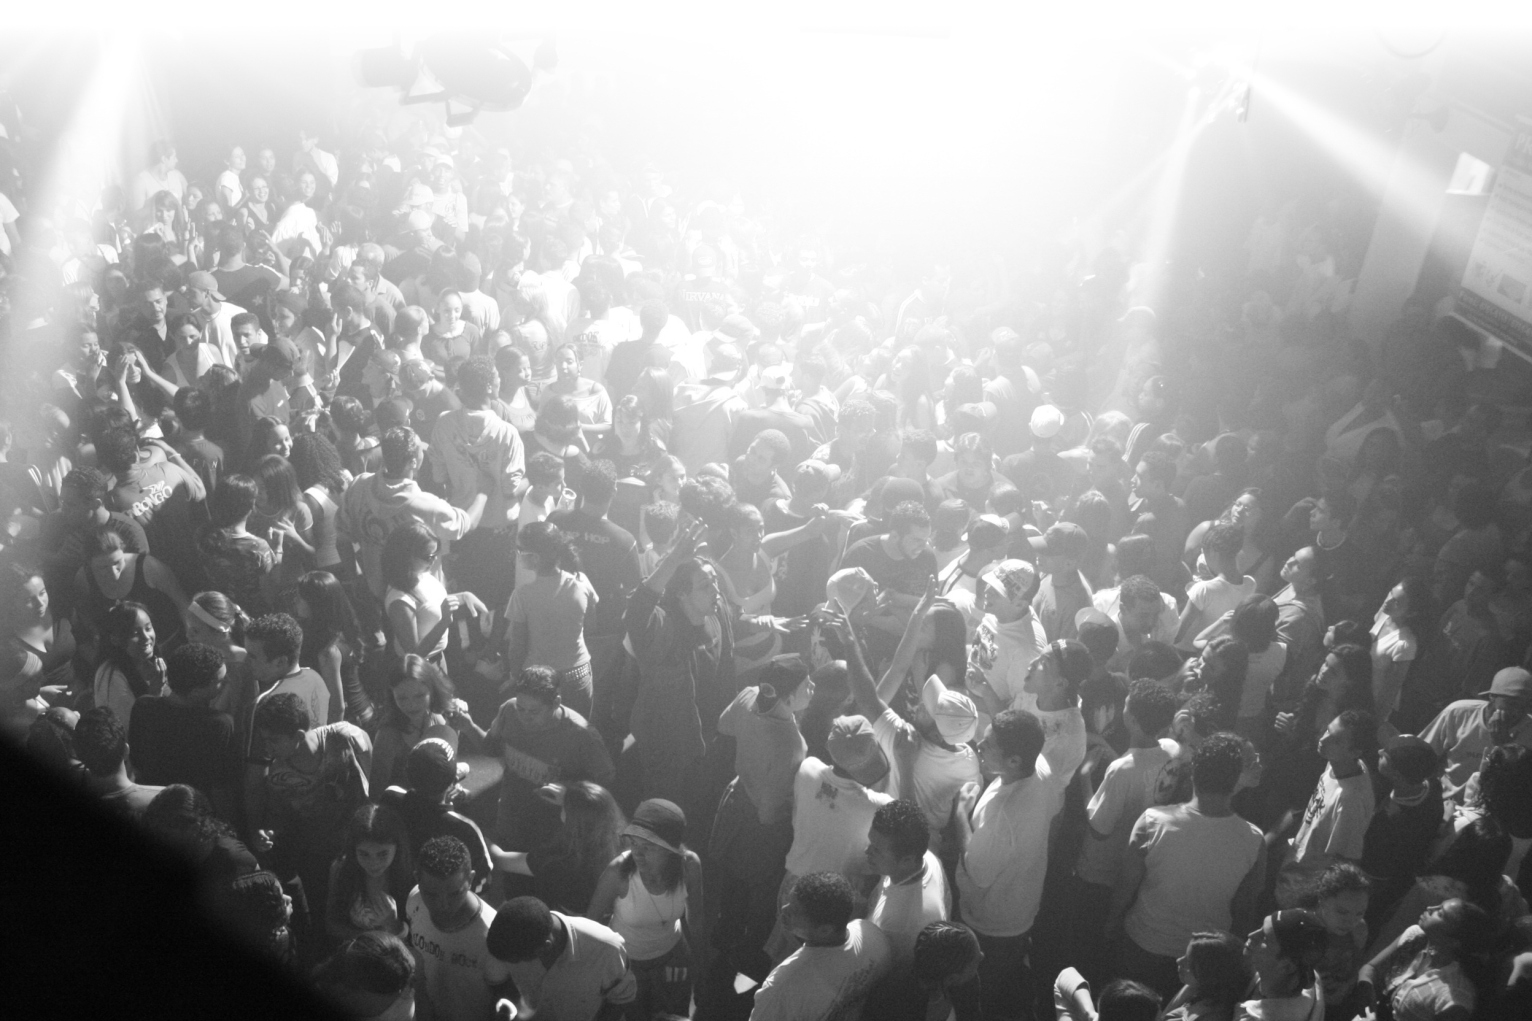
\includegraphics[scale=0.15,keepaspectratio=true]{img/imgs/7-diversao/-053.jpg}
\end{figure}

\begin{itemize}
\item   \textbf{Cooperativa Brasil:} Para quem gosta de um bom forró, sempre com
        shows diversos. A galera gosta muito da quarta-universitária.
        \\Site: \url{cooperativabrasil.com.br}.

\item   \textbf{Campinas Hall:} Muitas das festas mais legais da Unicamp
        acontecem lá (como a Festa Brega e a Festa do Contrário), perto da PUCC.
        É bem grande.

\item   \textbf{Delta Blues Bar:} O melhor do Blues \& Rock 'n Roll de
        Campinas.
        \\Site: \url{deltabluesbar.com.br}.

\item   \textbf{Swingers:} Tem bebidas caras e cada noite tem um tema, mas
        é melhor às quartas e quintas-feiras. Só homens maiores de 21 e mulheres
        com mais de 18 anos podem entrar.

\item   \textbf{Golden:} Assim como a Swingers fica no Shopping D. Pedro. Balada
        cara, frequentada geralmente por gente mais velha.
        \\Site: \url{goldstreetbar.com.br}

\item   \textbf{Barril da Máfia:} Boate com música ao vivo.
        \\Site: \url{barrildamafia.com.br}.

\item   \textbf{Kraft:} Localizada próxima ao Taquaral (na Avenida Imperatriz
        Leopoldina), toca musica psi a noite toda e fica aberta até quase
        o amanhecer. Mulher entra de graça até a meia-noite.

\item   \textbf{Cambuí:} Neste bairro existem diversos barzinhos, a maioria
        é temático, alguns são um pouco caros e cobram covert. É um ótima escolha
        para quem tiver carro pois fica um pouco longe de Barão.

\end{itemize}

\subsection{Shopping Centers}

\begin{figure}[h!]
    \centering
    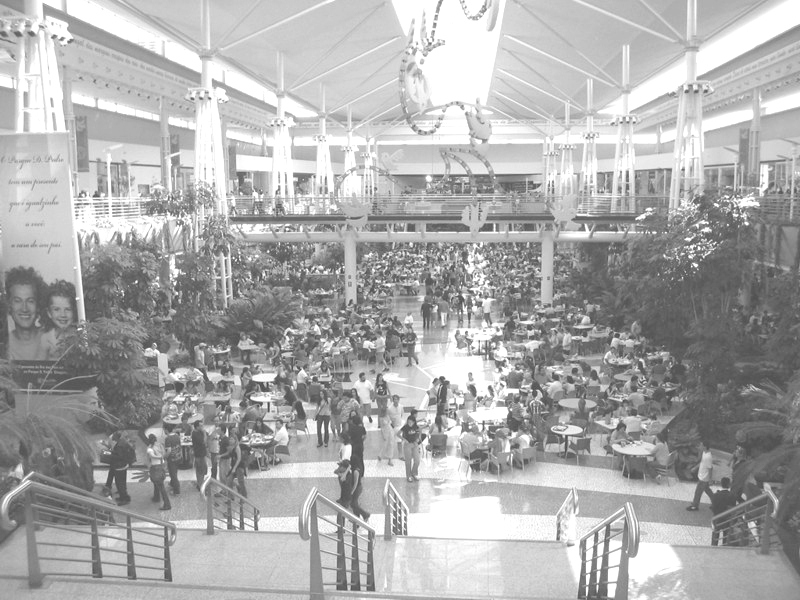
\includegraphics[scale=0.28,keepaspectratio=true]{img/imgs/7-diversao/-057.jpg}
\end{figure}

\begin{itemize}

\item   \textbf{Shopping Parque D. Pedro:} Foi considerado o maior shopping da
        América Latina até pouco tempo atrás. Localiza-se na Rodovia Dom Pedro,
        km 137 (razoavelmente próximo à Unicamp). O ônibus 3.38, que sai do
        Terminal Barão, vai para lá e para o Iguatemi. Outras opções de ônibus
        saindo do terminal são 2.10 e 3.00.
        \\Site: \url{parquedpedro.com.br}.

\item   \textbf{Shopping Iguatemi:} Shopping normal, o mais antigo e o segundo
        maior de Campinas. Localiza-se na Avenida Iguatemi, 777. O 3.38 demora
        uns 40 minutos para chegar lá. Frequentado pela galera mais nova e pelo
        pessoal com um pouco mais de dinheiro.
        \\Site: \url{www.iguatemicampinas.com.br}.

\item   \textbf{Parque das Bandeiras Shopping:} Inaugurado no fim de 2012.
        Localiza-se no Campo Grande, zona oeste de Campinas -- longe. Conta com
        telas de cinema de 300 m$^{2}$.
        \\Site: \url{shoppingparquedasbandeiras.com.br}.

\item   \textbf{Shopping Jaraguá:} Shopping pequeno e que possui duas unidades:
        Uma delas fica na Rua Conceiçao (Jaraguá Conceição) e a outra fica na
        avenida Brasil (Jaraguá Brasil). Nesse segundo há duas salas de cinema
        que passam filmes cult. O ônibus 3.30, no sentido Terminal
        Central--Unicamp, para razoavelmente próximo ao Jaraguá Conceição, um
        ponto antes do ponto da prefeitura; e os ônibus 3.30, 3.31, 3.32 e 3.33
        passam em frente ao Jaraguá Brasil.

\item   \textbf{Campinas Shopping:} Longe a dar com pau, mas as lojas não são
        muito caras. Localiza-se às margens das rodovias Anhanguera e Santos
        Dumont. Provavelmente você nunca irá lá.
        \\Site: \url{campinasshopping.com.br}.

\item   \textbf{Shopping Prado:} Shopping bem pequeno. As lojas não são muito
        caras, mas muito longe. Localiza-se na Avenida Washington Luís, 2480.
        Provavelmente você também nunca irá lá.

\item   \textbf{Galleria Shopping:} Muito bonito, mas lojas muito caras. Também
        localizado na Rodovia Dom Pedro, mas no km 131,5. O ônibus 3.00 sai do
        terminal de Barão Geraldo e passa lá.
        \\Site: \url{www.galleria.com.br}.

\item   \textbf{Shopping Unimart:} Shopping pequeno, as lojas não são muito
        caras. Localiza-se na Avenida John Boyd Dunlop, 350. O ônibus 1.34 sai
        do terminal de Barão Geraldo e passa próximo.
        \\Site: \url{unimart.com.br}.

\end{itemize}
